\documentclass[12pt]{article}
\usepackage{amsmath}
\usepackage{amssymb}
\usepackage{geometry}
\usepackage{amsmath, amsfonts, bm, graphicx}
\usepackage{tabularx}
\usepackage{booktabs} 
\usepackage{float}
\usepackage{enumitem}
\geometry{margin=1in}

\title{}
\date{}
\author{}

\begin{document}
\subsection*{\boxed{\text{HW 1 - Zeshui Song}}}

\section*{2.16}
\vspace{-3.5em}
\begin{figure}[H]
    \centering
    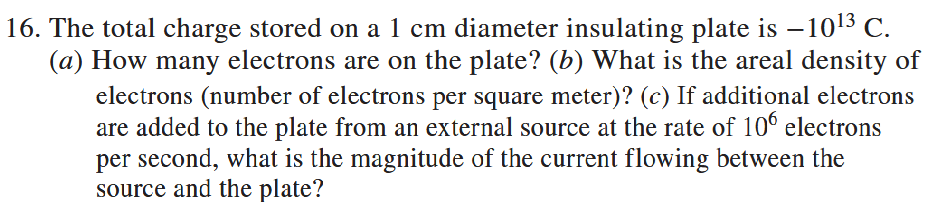
\includegraphics[width=0.8\textwidth]{2-16.png}
\end{figure}
\vspace{-1em}
\textbf{(a)}
\[[-10^{13}\,\text{C}]\left[\frac{\text{e}}{1.602 \times 10^{-19}\,\text{C}}\right] = -6.242 \times 10^{31}\,\text{e} \implies \boxed{6.242 \times 10^{31}\,\text{electrons}}\]
\textbf{(b)}
\[\sigma = \frac{6.242 \times 10^{31}\,\text{electrons}}{\frac{1}{4}\pi (10^{-2}\,\text{m})^2} = \boxed{7.947 \times 10^{35}\,\text{electrons/m}^2}\]
\textbf{(c)}
\[i = \frac{dq}{dt} = \frac{[10^6\,\text{electrons}][1.602 \times 10^{-19}\,\text{C/electron}]}{1\,\text{s}} = \boxed{1.602 \times 10^{-13}\,\text{C/s}}\]

\section*{2.25}
\vspace{-3.5em}
\begin{figure}[H]
    \centering
    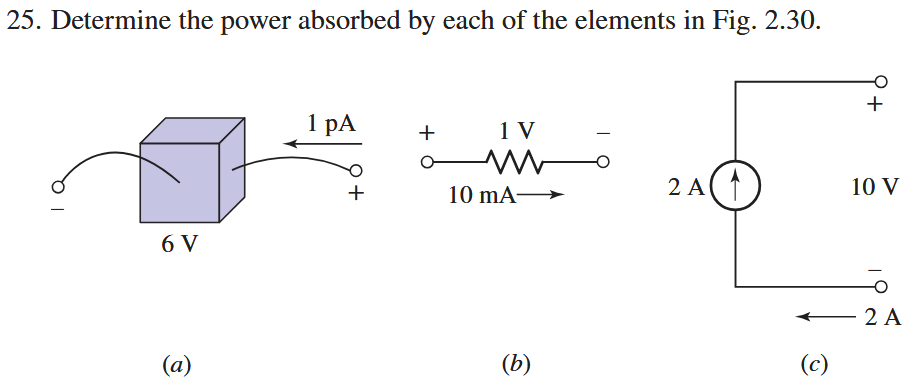
\includegraphics[width=0.8\textwidth]{2-25.png}
\end{figure}
\vspace{-1em}
\textbf{(a)}
\[P=[6\,\text{V}][1\times 10^{-12}\,\text{A}]=\boxed{6 \times 10^{-12}\,\text{W}}\]
\textbf{(b)}
\[P = [1\,\text{V}][10\times10^{-3}\,\text{A}] = \boxed{0.01\,\text{W}}\]
\textbf{(c)} The element is supplying 20 W of power.
\[P = [10\,\text{V}][-2\,\text{A}] = \boxed{-20\,\text{W}}\]
\underline{Note:} The sign convention is that if current enters the positive terminal, then power is being delivered or absorbed. If current enters the negative terminal, then power is being generated or supplied. Also, power is given by \(P = VI\).

\section*{2.30}
\vspace{-3.5em}
\begin{figure}[H]
    \centering
    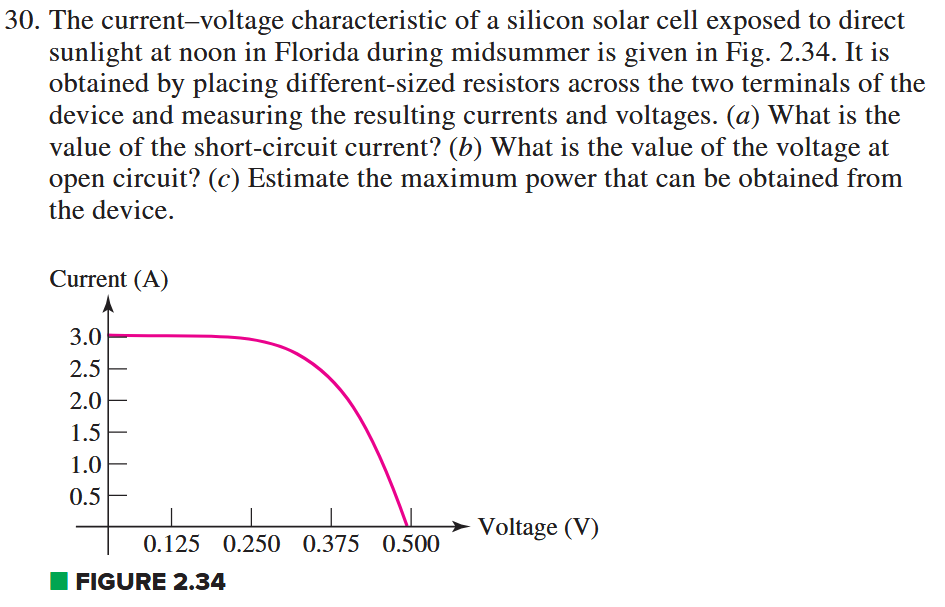
\includegraphics[width=0.8\textwidth]{2-30.png}
\end{figure}
\vspace{-1em}
\textbf{(a)} \boxed{3.0\,\text{A (short circuit)}}\\\\
\textbf{(b)} \boxed{0.500\,\text{V (open circuit)}}\\\\
\textbf{(c)} For maximum power, the product of current and voltage is max, this seems to happen around 0.375 V.
\[P_{max}=[0.375\,\text{V}][2.5\,\text{A}]=\boxed{0.9375\,\text{W}}\]
\underline{Note:} A \textbf{short circuit} is defined as a wire with zero resistance, and thus corresponds to a voltage of 0 V across its terminals. An \textbf{open circuit} is defined as a break in the circuit with infinite resistance, and thus corresponds to a current of 0 A through its terminals.

\section*{2.35}
\vspace{-3.5em}
\begin{figure}[H]
    \centering
    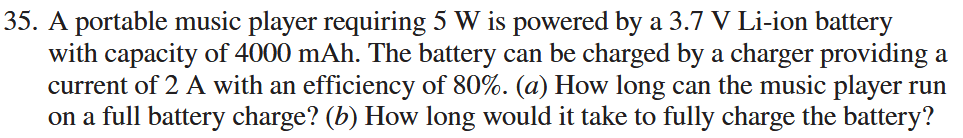
\includegraphics[width=0.8\textwidth]{2-35.png}
\end{figure}
\vspace{-1em}
\textbf{(a)}
\[w = [3.7\,\text{W}][4000\times10^{-3}\,\text{Ah}] = 14.8\,\text{Wh}\]
\[t = \frac{[14.8\,\text{Wh}]}{[5\,\text{W}]} = \boxed{2.96\,\text{h}}\]
\textbf{(b)}
\[I_{eff} = [2\,\text{A}][0.8] = 1.6\,\text{A}\]
\[t = \frac{[4000\times10^{-3}\,\text{Ah}]}{[1.6\,\text{A}]} = \boxed{2.5\,\text{h}}\]
\underline{Note:} Recall that work is the product of power and time, thus energy is given by $\boxed{1\,\text{J} = 1\,\text{W} \times 1\,\text{s}}$. Energy is usually measured in \textbf{watt hours (Wh)} where \boxed{1\,\text{Wh} = 3600\,\text{J}}.\\\\
\textbf{Battery capacity} (energy stored) is then also given in terms of Wh. Since the voltage of a battery is constant, we can define the energy stored in terms of the charge capacity $Q$ (in Ampere hours, Ah) and voltage $V$ (in Volts, V) as:
\[w = \int P\,dt = \int VI\,dt = V\int I\,dt = VQ\]
where $Q$ is in Ah, $V$ is in V, and $w$ is in Wh.\\\\
To find how long the battery will last, we can divide its battery capacity by the load/output power.
\[t = \frac{w}{P}\]
To find how long it will take to charge the battery, we can divide its charge capacity by the charging current.
\[t = \frac{Q}{I_{eff}}\]
Where $I_{eff}$ is the effective charging current accounting for any losses ($I_{eff} = I_{in} \times \eta$ where $\eta$ is the efficiency of the charger).

\section*{2.40}
\vspace{-3.5em}
\begin{figure}[H]
    \centering
    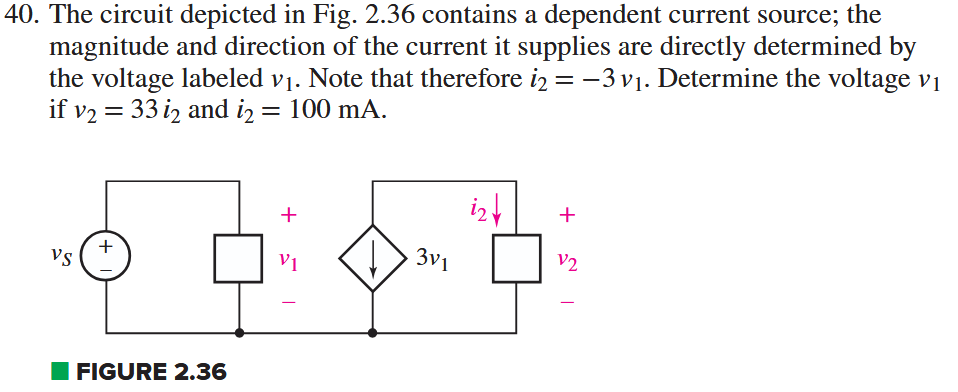
\includegraphics[width=0.8\textwidth]{2-40.png}
\end{figure}
\vspace{-1em}
\[i_2 = -3v_1 = [100\times10^{-3}\,\text{A}]\]
\[\implies v_1 = \frac{-100\times10^{-3}\,\text{A}}{3} = \boxed{-33.3 \times 10^{-3}\,\text{V}}\]
\underline{Note:} The diamond shaped symbol represents a \textbf{voltage dependent current source} with current direction indicated by the arrow. By conservation of charge, $i_2$ must be equal in magnitude and direction, which is why is it set equal to $-3v_1$.

\section*{2.43}
\vspace{-3.5em}
\begin{figure}[H]
    \centering
    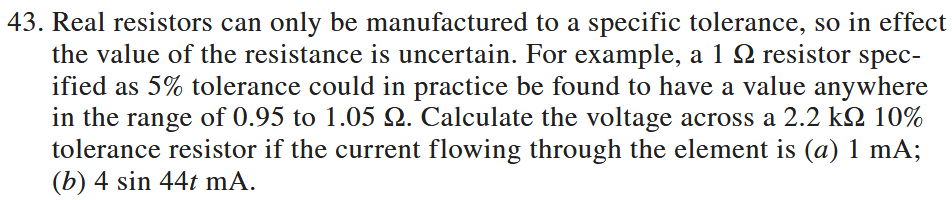
\includegraphics[width=0.8\textwidth]{2-43.png}
\end{figure}
\vspace{-1em}
\[\text{Tolerance} = 0.1 \times [2.2\times10^{3}\,\Omega] = 220\,\Omega\]
\[R = 2.2 \times 10^{3} \pm 220\,\Omega\]
\textbf{(a)}
\[V = [1\times10^{-3}\,\text{A}][2.2 \times 10^{3}\,\Omega] = 2.2\,\text{V}\]
\[\Delta V = [1\times10^{-3}\,\text{A}][220\,\Omega] = 0.22\,\text{V}\]
\[\implies \boxed{V = 2.2 \pm 0.22\,\text{V}}\]
\textbf{(b)}
\[V = [4sin(44t)\,\text{A}][2.2 \times 10^{3}\,\Omega] = 8.8sin(44t)\,\text{V}\]
\[\Delta V = [4sin(44t)\,\text{A}][220\,\Omega] = 0.88sin(44t)\,\text{V}\]
\[\implies \boxed{V = 8.8sin(44t) \pm 0.88sin(44t)\,\text{V}}\]

\section*{2.53}
\vspace{-3.5em}
\begin{figure}[H]
    \centering
    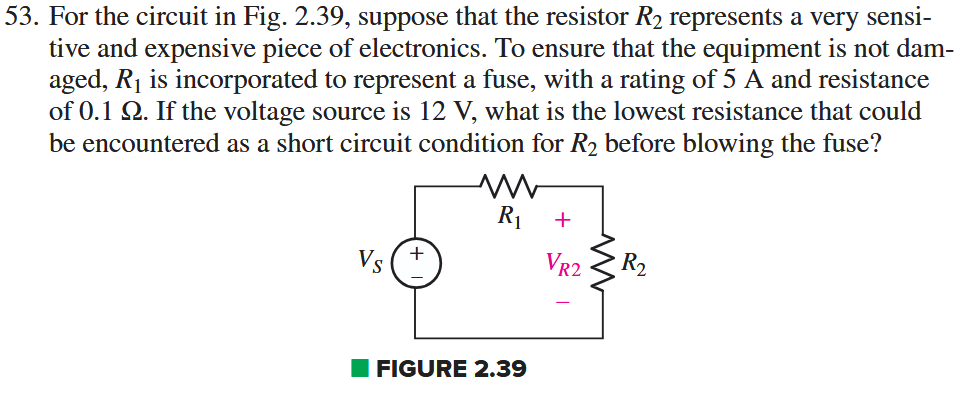
\includegraphics[width=0.8\textwidth]{2-53.png}
\end{figure}
\vspace{-1em}
\[V=I_{max}R_{eq} \implies R_{eq} = \frac{[12\,\text{V}]}{[5\,\text{A}]}=2.4\,\Omega\]
\[R_{eq} = R_1 + R_2 \implies R_2 = R_{eq} - R_1\]
\[R_2 = [2.4\,\Omega] - [0.1\,\Omega] = \boxed{2.3\,\Omega}\]
\underline{Note:} Any increase in $R_2$ will cause the current to be below 5 A, and any decrease in $R_2$ will cause the fuse to blow.

\section*{2.60}
\vspace{-3.5em}
\begin{figure}[H]
    \centering
    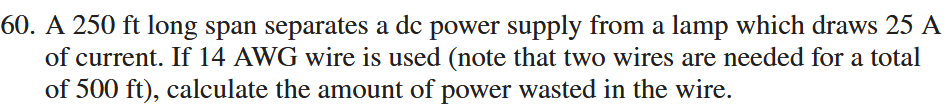
\includegraphics[width=0.8\textwidth]{2-60.png}
\end{figure}
\vspace{-1em}
14 AWG wire: 2.08 $\text{mm}^2$ cross-sectional area, 2.52 Ohms per 1000 ft at 20$^\circ$C
\[R = [\,2.52\,\Omega/(1000\,\text{ft})\,]\,[1/2\,(1000\,\text{ft})]
  = 1.26\,\Omega\]
\[P_{loss} = I^2 R = [25\,\text{A}]^2 [1.26\,\Omega] = \boxed{787.5\,\text{W}}\]
\underline{Note:} AWG refers to the American Wire Gauge standard for wire diameters. The larger the AWG number, the smaller the diameter of the wire.

\section*{3.5}
\vspace{-3.5em}
\begin{figure}[H]
    \centering
    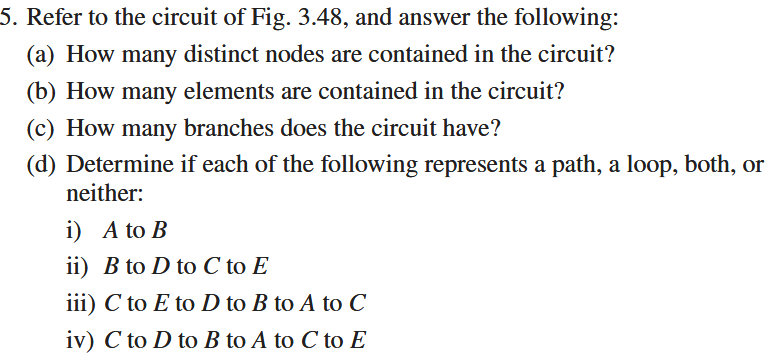
\includegraphics[width=0.8\textwidth]{3-5.png}
\end{figure}
\vspace{-2em}
\begin{figure}[H]
    \centering
    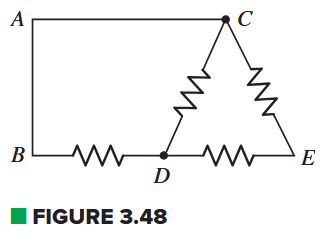
\includegraphics[width=0.4\textwidth]{3-5_1.png}
\end{figure}
\vspace{-1em}
\textbf{(a)} \boxed{\text{4 nodes:} B, C, D, E}\\\\
\underline{Note:} A \textbf{node} is a point in a circuit where two or more circuit elements meet.\\\\
\textbf{(b)} \boxed{\text{4 elements}}\\\\
\textbf{(c)} \boxed{\text{4 branches: }BD,DE,CE,CD}\\\\
\underline{Note:} A \textbf{branch} is a single circuit element connected between two nodes.\\\\
\textbf{(d)}
\begin{enumerate}[label=\roman*)]
  \item Path
  \item Path
  \item Loop
  \item Neither
\end{enumerate}
\underline{Note:} A \textbf{path} is a sequence of connected elements that does not pass through any node more than once.
If the path starts and ends at the same node, it is a \textbf{loop}.

\section*{3.10}
\vspace{-3.5em}
\begin{figure}[H]
    \centering
    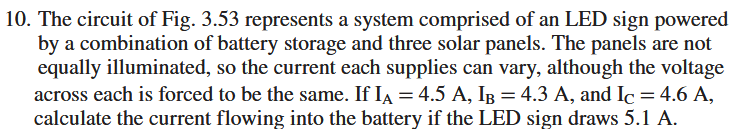
\includegraphics[width=0.8\textwidth]{3-10.png}
\end{figure}
\vspace{-2em}
\begin{figure}[H]
    \centering
    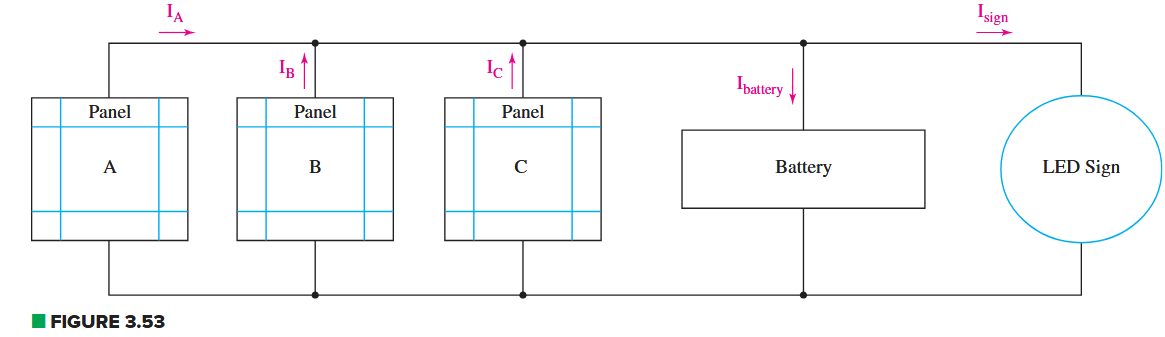
\includegraphics[width=1\textwidth]{3-10_1.png}
\end{figure}
\vspace{-1em}
Given:
\begin{itemize}
  \item $I_A = 4.5\,\text{A}$
  \item $I_B = 4.3\,\text{A}$
  \item $I_C = 4.6\,\text{A}$
  \item $I_{\text{sign}} = 5.1\,\text{A}$
\end{itemize}
Using Kirchhoff's Current Law (KCL) at the node above the battery:
\[I_A+I_B+I_C=I_{\text{battery}}+I_{\text{sign}}\]
\[\implies I_{\text{battery}} = I_A + I_B + I_C - I_{\text{sign}}\]
\[\implies I_{\text{battery}} = [4.5 + 4.3 + 4.6 - 5.1]\,\text{A} = \boxed{8.3\,\text{A}}\]

\section*{3.12}
\vspace{-3.5em}
\begin{figure}[H]
    \centering
    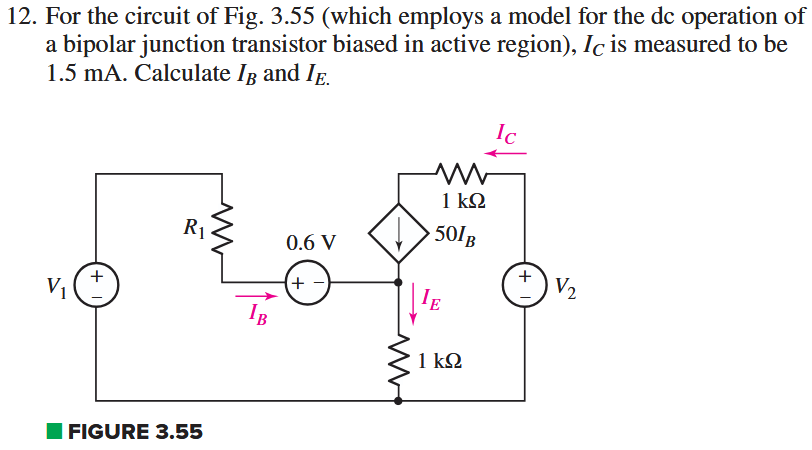
\includegraphics[width=0.8\textwidth]{3-12.png}
\end{figure}
\vspace{-1em}
Using Kirchhoff's Current Law (KCL) at the node before the current source:
\[I_C = 50I_B \implies I_B = \frac{[1.5\,\text{mA}]}{50}=\boxed{0.03\,\text{mA}}\]
Using KCL at the node below the current source:
\[I_B + I_C = I_E\]
\[\implies I_E = [0.03 + 1.5]\,\text{mA} = \boxed{1.53\,\text{mA}}\]

\section*{3.20}
\vspace{-3.5em}
\begin{figure}[H]
    \centering
    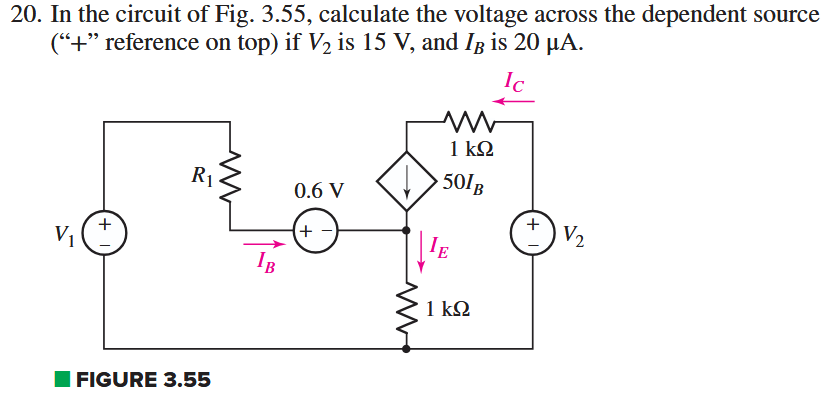
\includegraphics[width=0.8\textwidth]{3-20.png}
\end{figure}
\vspace{-1em}
Using KCL at the node before the current source:
\[I_C = 50I_B=50[20\times10^{-6}\,\text{A}]=1\times10^{-3}\,\text{A}\]
Using KCL at the node after the current source:
\[I_B + I_C = I_E\]
\[\implies I_E = [20\times10^{-6} + 1\times10^{-3}]\,\text{A} = 1.02\times10^{-3}\,\text{A}\]
Using Kirchhoff's Voltage Law (KVL) around the loop containing the current source:
\[-V_{\text{source}}-[1\times10^3\,\Omega]I_E+V_2-[1\times10^3\,\Omega]I_C =0\]
\[\implies V_{\text{source}} = -[1\times10^3\,\Omega][1.02\times10^{-3}\,\text{A}] + [15\,\text{V}] - [1\times10^3\,\Omega][1\times10^{-3}\,\text{A}]\]
\[\boxed{V_{\text{source}} = 12.98\,\text{V}}\]

\end{document}